\documentclass[a4paper, UTF-8]{article}
\usepackage{algorithm}
\usepackage{algpseudocode}
\usepackage{amsmath}
\usepackage{amsfonts}
\usepackage{amsthm}
\usepackage{tikz}
\usetikzlibrary{automata, positioning, arrows, trees}
\usepackage[utf8]{inputenc} % allow utf-8 input
\usepackage[T1]{fontenc}    % use 8-bit T1 fonts
\usepackage{hyperref}       % hyperlinks
\usepackage{url}            % simple URL typesetting
\usepackage{booktabs}       % professional-quality tables
\usepackage{amsfonts}       % blackboard math symbols
\usepackage{nicefrac}       % compact symbols for 1/2, etc.
\usepackage{microtype}      % microtypography
\usepackage{xcolor}         % colors

\theoremstyle{plain}
\newtheorem{theorem}{\indent Theorem}[section]
\newtheorem{lemma}[theorem]{\indent Lemma}
\newtheorem{assumption}{\indent Assumption}[section]
\newtheorem{note}[theorem]{\indent Notation}
\newtheorem{proposition}[theorem]{\indent Proposition}
\newtheorem{corollary}[theorem]{\indent Corollary}
\newtheorem{definition}{\indent Definition}[section]
\newtheorem{example}{\indent Example}[section]
\newtheorem{remark}{\indent Remark}[section]
\newenvironment{solution}{\begin{proof}[\indent\bf Solution]}{\end{proof}}
\renewcommand{\proofname}{\indent\bf Proof}

\begin{document}

\title{\bf{Lab6 Answers}}

\author{Yanqiao Chen*\\ 
  Department of Computer Science and Engineering\\
  Southern University of Science and Technology\\
  \texttt{12412115@mail.sustech.edu.cn}
  }

\maketitle

\section{Question 1} 

\subsection{a)} 

Let us create three states $q_{start}, q_{loop}, q_{end}$. From $q_{start} $, we first push \$ and then $E$ into the stack. Then for each substitution rule, we create the following transitions: 
\begin{itemize}
    \item $\epsilon, E \to T/\epsilon, \epsilon \to +/\epsilon, \epsilon \to E$ 
    \item $\epsilon, E \to T$ 
    \item $\epsilon, T \to F/ \epsilon, \epsilon \to \times/ \epsilon, \epsilon \to T$ 
    \item $\epsilon, T \to F$ 
    \item $\epsilon, F \to ) / \epsilon, \epsilon \to E/ \epsilon, \epsilon \to (/ \epsilon$
    \item $\epsilon, F \to a$ 
    \item $a, a \to epsilon$ 
\end{itemize} 
Finally, we create a transition from $q_{loop}$ to $q_{end}$ when the stack is empty and the input is \$.

We may draw the PDA as follows:

\begin{center}
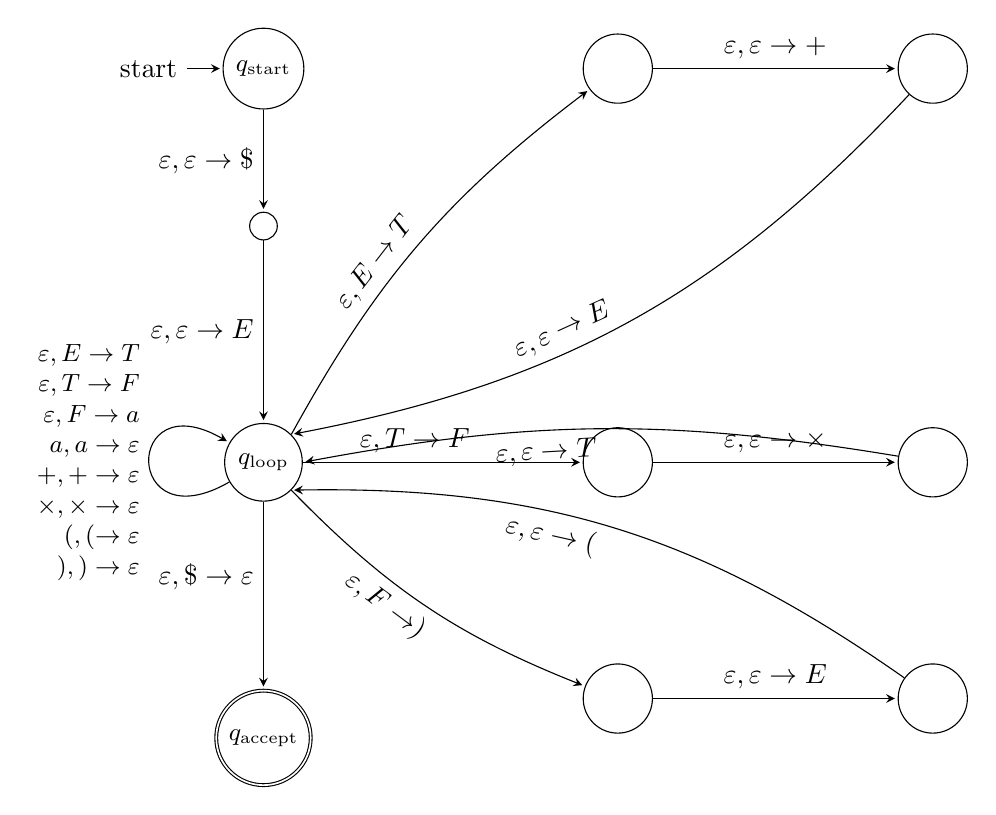
\begin{tikzpicture}[shorten >=1pt, >=stealth,
  every state/.style={font=\small}
]
  % Main vertical states on the left
  \node[state, initial] (qs) at (0,5) {$q_{\text{start}}$};
  \node[state, inner sep=1pt, minimum size=10pt] (qmid) at (0,3) {};
  \node[state] (ql) at (0,0) {$q_{\text{loop}}$};
  \node[state, accepting] (qa) at (0,-3.5) {$q_{\text{accept}}$};

  % Intermediate states on the right (spread out)
  \node[state] (e1) at (4.5,5) {};
  \node[state] (e2) at (8.5,5) {};
  \node[state] (t1) at (4.5,0) {};
  \node[state] (t2) at (8.5,0) {};
  \node[state] (f1) at (4.5,-3) {};
  \node[state] (f2) at (8.5,-3) {};

  % Vertical transitions
  \draw[->] (qs) -- node[left] {$\varepsilon,\varepsilon\to \$$} (qmid);
  \draw[->] (qmid) -- node[left] {$\varepsilon,\varepsilon\to E$} (ql);
  \draw[->] (ql) -- node[left, pos=0.4] {$\varepsilon,\$\to\varepsilon$} (qa);

  % E -> E+T
  \draw[->] (ql.north east) to[bend left=12] node[above, sloped, pos=0.4] {$\varepsilon,E\to T$} (e1);
  \draw[->] (e1) -- node[above] {$\varepsilon,\varepsilon\to +$} (e2);
  \draw[->] (e2) to[bend left=18] node[above, sloped, pos=0.6] {$\varepsilon,\varepsilon\to E$} (ql.north east);

  % T -> T*F
  \draw[->] (ql.east) to node[above, sloped, pos=0.4] {$\varepsilon,T\to F$} (t1);
  \draw[->] (t1) -- node[above] {$\varepsilon,\varepsilon\to \times$} (t2);
  \draw[->] (t2) to[bend right=10] node[below, sloped, pos=0.6] {$\varepsilon,\varepsilon\to T$} (ql.east);

  % F -> (E)
  \draw[->] (ql.south east) to[bend right=12] node[below, sloped, pos=0.4] {$\varepsilon,F\to )$} (f1);
  \draw[->] (f1) -- node[above] {$\varepsilon,\varepsilon\to E$} (f2);
  \draw[->] (f2) to[bend right=18] node[below, sloped, pos=0.6] {$\varepsilon,\varepsilon\to ($} (ql.south east);

  % Self-loop on the left
  \path[->] (ql) edge[loop left, min distance=12mm, in=150, out=210, looseness=8]
    node[left, font=\small, align=right] {
      $\varepsilon,E\to T$\\
      $\varepsilon,T\to F$\\
      $\varepsilon,F\to a$\\
      $a,a\to\varepsilon$\\
      $+,+\to\varepsilon$\\
      $\times,\times\to\varepsilon$\\
      $(,(\to\varepsilon$\\
      $),)\to\varepsilon$
    } (ql);
\end{tikzpicture}
\end{center}



\subsection{b)}

We create four main states $q_{\text{start}}$, a small intermediate state, $q_{\text{loop}}$, and $q_{\text{accept}}$. From $q_{\text{start}}$ we first push $\$$ and then $R$ into the stack. For each substitution rule we obtain the following transitions (multi-push rules are split into paths through intermediate states):
\begin{itemize}
    \item $\varepsilon, R \to X / \varepsilon, \varepsilon \to R / \varepsilon, \varepsilon \to X$
    \item $\varepsilon, R \to S$
    \item $\varepsilon, S \to b / \varepsilon, \varepsilon \to T / \varepsilon, \varepsilon \to a$
    \item $\varepsilon, S \to a / \varepsilon, \varepsilon \to T / \varepsilon, \varepsilon \to b$
    \item $\varepsilon, T \to X / \varepsilon, \varepsilon \to T / \varepsilon, \varepsilon \to X$
    \item $\varepsilon, T \to X$
    \item $\varepsilon, T \to \varepsilon$
    \item $\varepsilon, X \to a$
    \item $\varepsilon, X \to b$
    \item $a, a \to \varepsilon$ \quad $b, b \to \varepsilon$
\end{itemize}
Finally we transition from $q_{\text{loop}}$ to $q_{\text{accept}}$ on $\varepsilon, \$ \to \varepsilon$.

\begin{center}
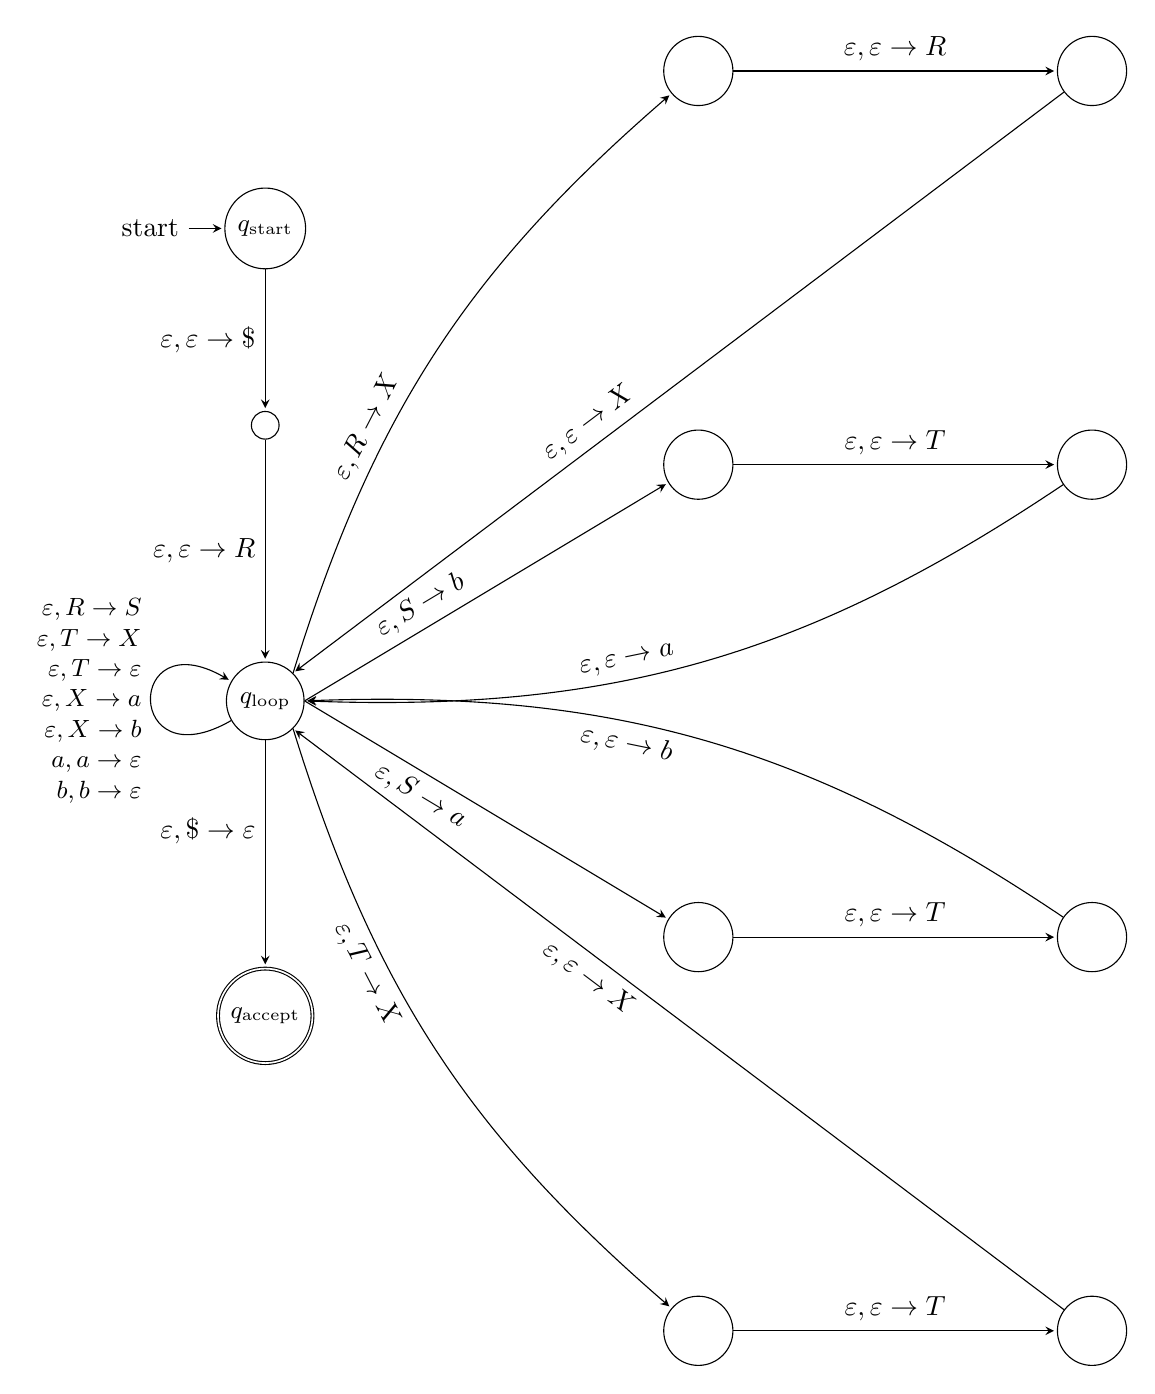
\begin{tikzpicture}[shorten >=1pt, >=stealth,
  every state/.style={font=\small}
]
  % Main vertical states on the left
  \node[state, initial] (qs) at (0,6) {$q_{\text{start}}$};
  \node[state, inner sep=1pt, minimum size=10pt] (qmid) at (0,3.5) {};
  \node[state] (ql) at (0,0) {$q_{\text{loop}}$};
  \node[state, accepting] (qa) at (0,-4) {$q_{\text{accept}}$};

  % Intermediate states on the right (spread out)
  \node[state] (r1) at (5.5,8) {};
  \node[state] (r2) at (10.5,8) {};
  \node[state] (s1a) at (5.5,3) {};
  \node[state] (s2a) at (10.5,3) {};
  \node[state] (s1b) at (5.5,-3) {};
  \node[state] (s2b) at (10.5,-3) {};
  \node[state] (t1) at (5.5,-8) {};
  \node[state] (t2) at (10.5,-8) {};

  % Vertical transitions
  \draw[->] (qs) -- node[left] {$\varepsilon,\varepsilon\to \$$} (qmid);
  \draw[->] (qmid) -- node[left] {$\varepsilon,\varepsilon\to R$} (ql);
  \draw[->] (ql) -- node[left, pos=0.4] {$\varepsilon,\$\to\varepsilon$} (qa);

  % R -> XRX
  \draw[->] (ql.north east) to[bend left=16] node[above, sloped, pos=0.35] {$\varepsilon,R\to X$} (r1);
  \draw[->] (r1) -- node[above] {$\varepsilon,\varepsilon\to R$} (r2);
  \draw[->] (r2) to node[above, sloped, pos=0.6] {$\varepsilon,\varepsilon\to X$} (ql.north east);

  % S -> aTb
  \draw[->] (ql.east) to node[above, sloped, pos=0.35] {$\varepsilon,S\to b$} (s1a);
  \draw[->] (s1a) -- node[above] {$\varepsilon,\varepsilon\to T$} (s2a);
  \draw[->] (s2a) to[bend left=18] node[above, sloped, pos=0.6] {$\varepsilon,\varepsilon\to a$} (ql.east);

  % S -> bTa
  \draw[->] (ql.east) to node[below, sloped, pos=0.35] {$\varepsilon,S\to a$} (s1b);
  \draw[->] (s1b) -- node[above] {$\varepsilon,\varepsilon\to T$} (s2b);
  \draw[->] (s2b) to[bend right=18] node[below, sloped, pos=0.6] {$\varepsilon,\varepsilon\to b$} (ql.east);

  % T -> XTX
  \draw[->] (ql.south east) to[bend right=16] node[below, sloped, pos=0.35] {$\varepsilon,T\to X$} (t1);
  \draw[->] (t1) -- node[above] {$\varepsilon,\varepsilon\to T$} (t2);
  \draw[->] (t2) to node[below, sloped, pos=0.6] {$\varepsilon,\varepsilon\to X$} (ql.south east);

  % Self-loop on the left
  \path[->] (ql) edge[loop left, min distance=12mm, in=150, out=210, looseness=8]
    node[left, font=\small, align=right] {
      $\varepsilon,R\to S$\\
      $\varepsilon,T\to X$\\
      $\varepsilon,T\to\varepsilon$\\
      $\varepsilon,X\to a$\\
      $\varepsilon,X\to b$\\
      $a,a\to\varepsilon$\\
      $b,b\to\varepsilon$
    } (ql);
\end{tikzpicture}
\end{center}

\section{Question 2}

First we check that there is only one accept state ($q_4$) and that the stack is empty before entering the accept state.

The complete CFG is constructed as follows (using the standard PDA-to-CFG construction):
\begin{enumerate}
    \item For every state $p \in \{q_1,q_2,q_3,q_4\}$, add the base rule
    \[
        A_{pp} \to \varepsilon .
    \]
    \item For every triple of states $p,q,r \in \{q_1,q_2,q_3,q_4\}$, add the concatenation rule
    \[
        A_{pq} \to A_{pr}A_{rq} .
    \]
    \item For every matched pair of a push transition and a pop transition on the same stack symbol $t$, add the corresponding rule $A_{pq} \to a A_{rs} b$:
    \begin{itemize}
        \item Push $\$$ at $q_1 \xrightarrow{\varepsilon,\varepsilon\to\$} q_2$ and pop $\$$ at $q_3 \xrightarrow{\varepsilon,\$\to\varepsilon} q_4$:
        \[
            A_{q_1q_4} \to \varepsilon A_{q_2q_3} \varepsilon ;
        \]
        \item Push $0$ at $q_2 \xrightarrow{0,\varepsilon\to 0} q_2$ and pop $0$ at $q_3 \xrightarrow{0,0\to\varepsilon} q_3$:
        \[
            A_{q_2q_3} \to 0 A_{q_2q_3} 0 ;
        \]
        \item Push $1$ at $q_2 \xrightarrow{1,\varepsilon\to 1} q_2$ and pop $1$ at $q_3 \xrightarrow{1,1\to\varepsilon} q_3$:
        \[
            A_{q_2q_3} \to 1 A_{q_2q_3} 1 .
        \]
    \end{itemize}
    \item The transition $q_2 \xrightarrow{\varepsilon,\varepsilon\to\varepsilon} q_3$ neither pushes nor pops, so it contributes
    \[
        A_{q_2q_3} \to \varepsilon .
    \]
\end{enumerate}

In summary, the complete CFG is:
\begin{align*}
    A_{q_1q_1} &\to \varepsilon \\[-3pt]
    A_{q_2q_2} &\to \varepsilon \\[-3pt]
    A_{q_3q_3} &\to \varepsilon \\[-3pt]
    A_{q_4q_4} &\to \varepsilon \\[2pt]
    A_{pq} &\to A_{pr}A_{rq} \quad (\forall p,q,r \in \{q_1,q_2,q_3,q_4\}) \\[2pt]
    A_{q_1q_4} &\to \varepsilon A_{q_2q_3} \varepsilon \\[-3pt]
    A_{q_2q_3} &\to 0 A_{q_2q_3} 0 \\[-3pt]
    A_{q_2q_3} &\to 1 A_{q_2q_3} 1 \\[-3pt]
    A_{q_2q_3} &\to \varepsilon
\end{align*}
where the start variable is $A_{q_1q_4}$.

\section{Question 3} 

The proof is similar to the proof in the regular language. 

For union, we can construct a new start state and add $\epsilon, \epsilon \to \mathdollar$ from the new start state to the start states of the two PDAs.

For concatenation, we can add $\epsilon, \epsilon \to \epsilon$ from the accept states of the first PDA to the start state of the second PDA.

For Kleene star, we can add $\epsilon, \epsilon \to \epsilon$ from the accept states to the start state, and add $\epsilon, \epsilon \to \epsilon$ from the new start state, which must be a accept state, to the old start state.

This shows that the class of languages recognized by PDAs is closed under union, concatenation, and Kleene star.

\section{Question 4} 

We prove this by induction. For the base case,
\begin{itemize}
    \item $\{\epsilon\}$ is context free, as it can be generated by the CFG with the single rule $S \to \epsilon$.
    \item $\{a\}, a\in \Sigma$ is context free, as it can be generated by the CFG with the single rule $S \to a$.
    \item $\emptyset$ is context free, as it can be generated by the CFG with the single rule $S \to S$.
\end{itemize}

From the Question 3, we know that the class of context free languages is closed under union, concatenation, and Kleene star. Therefore, if $L_1$ and $L_2$ are context free, then $L_1 \cup L_2$, $L_1 L_2$, and $L_1^*$ are also context free.

On the other hand, $R$ that is constructed by $a\in \Sigma, \epsilon, \emptyset$ under the three operations is exactly a regular expression. Thus, every regular expression is context free, which means that every regular language has an equivalent CFG.

\section{Question 5} 

For any string $w$, in every derivation of $w$ in a CFG in CNF, we can see that starting from a single variable $S$ with length 1 and each operation will extend the length by 1, the number of operations must be $|w|-1$. Then in the end, we need to apply the rule $A \to a$ for each symbol in $w$, which contributes $|w|$ operations. Therefore, the total number of operations is $2|w|-1$.

\section{Question 6}

\subsection{a)}

Let the pumping length be $p$. Consider the string $s = 0^p1^p0^p1^p \in L$. By the pumping lemma for CFLs, $s = uvxyz$ with $|vxy| \leq p$ and $|vy| \geq 1$.

Because $|vxy| \leq p$, the substring $vxy$ can intersect at most two consecutive blocks. Let $a_1,a_2,a_3,a_4$ denote the lengths of the four blocks of $0$s and $1$s in $uv^ixy^iz$, so initially $a_1=a_2=a_3=a_4=p$. After pumping to $i=2$, at least one block that intersects $vy$ strictly increases in length because $|vy| \geq 1$, while any untouched block stays at length $p$. Hence there exists some index $j$ with $a_j \geq p+1$ and at least one other index $k\neq j$ with $a_k = p$, so $a_j \neq a_k$. Therefore $uv^2xy^2z \notin \{0^n1^n0^n1^n \mid n \geq 0\}$, and $L$ is not context-free.

\subsection{b)}

Let the pumping length be $p$. Consider $s = 0^p\#0^{2p}\#0^{3p} \in L$. By the pumping lemma for CFLs, $s = uvxyz$ with $|vxy| \leq p$ and $|vy| \geq 1$.

Since $|vxy| \leq p$, $vxy$ cannot contain both $\#$ symbols and thus lies entirely within at most two consecutive $0$-segments. Let $b_1,b_2,b_3$ be the lengths of the three $0$-segments in $uv^ixy^iz$; initially $(b_1,b_2,b_3) = (p,2p,3p)$.

For instance, if $v$ and $y$ both lie inside the first segment, then after pumping to $i=2$ we obtain $(b_1',b_2',b_3') = (p+|vy|,2p,3p)$. If $b_1' = n$ for some $n$, then we would need $b_2' = 2n$ and $b_3' = 3n$, i.e. $2p = 2(p+|vy|)$, which implies $|vy| = 0$, contradicting $|vy| \geq 1$. The same argument applies when $vxy$ lies in any other one or two consecutive segments: at least one of the three equalities $b_2'=2b_1'$ and $b_3'=3b_2'$ (or equivalently $b_3'=3b_1'$) must fail. Thus $uv^2xy^2z \notin \{0^n\#0^{2n}\#0^{3n} \mid n \geq 0\}$, and $L$ is not context-free.

\section{Question 7} 

Notice that $A \cap B = \{a^mb^nc^n \mid m,n \geq 0\} \cap \{a^nb^nc^m \mid m,n \geq 0\} = \{a^nb^nc^n\}$. From the lecture we know that $\{a^nb^nc^n\}$ is not context-free, so $A \cap B$ is not context-free. We know that $\{b^nc^n\mid n \geq 0\}$ and $\{a^nb^n\mid n \geq 0\}$ are context-free, so by the closure properties of context-free languages under concatenation, $A$ and $B$ are context-free. Therefore, the class of context-free languages is not closed under intersection.

\section{Question 8}

We prove this by contradiction. Assume that the class of context-free languages is closed under complement. Let $L_1$ and $L_2$ be arbitrary context-free languages. Then $\overline{L_1}$ and $\overline{L_2}$ are also context-free by our assumption. Since context-free languages are closed under union, $\overline{L_1} \cup \overline{L_2}$ is context-free. Complementing again (by assumption), we obtain
\[
    \overline{\overline{L_1} \cup \overline{L_2}} = L_1 \cap L_2 ,
\]
which must therefore be context-free. This implies that context-free languages are closed under intersection, contradicting Question 7. Hence the class of context-free languages is not closed under complement.

\section{Question 9}

Let $P = (Q_C, \Sigma, \Gamma, \delta_C, s_C, Z_0, F_C)$ be a PDA that recognises the CFL $C$, and let $A = (Q_R, \Sigma, \delta_R, s_R, F_R)$ be a DFA that recognises the regular language $R$. We construct a new PDA $P'$ by taking the product of the state sets of $P$ and $A$:
\[
    P' = (Q_C \times Q_R,\; \Sigma,\; \Gamma,\; \delta',\; (s_C, s_R),\; Z_0,\; F_C \times F_R).
\]

Formally, the transition function $\delta' : (\Sigma \cup \{\varepsilon\}) \times (Q_C \times Q_R) \times \Gamma \to \mathcal{P}((Q_C \times Q_R) \times \Gamma^{*})$ is defined by: for all $q_C \in Q_C$, $q_R \in Q_R$, $X \in \Gamma$, and $a \in \Sigma$,
\begin{align*}
    \delta'(\varepsilon, (q_C, q_R), X) &= \big\{ ((p_C, q_R), \gamma) \mid (p_C, \gamma) \in \delta_C(\varepsilon, q_C, X) \big\}, \\
    \delta'(a, (q_C, q_R), X) &= \big\{ ((p_C, \delta_R(a, q_R)), \gamma) \mid (p_C, \gamma) \in \delta_C(a, q_C, X) \big\}.
\end{align*}

Intuitively, $P'$ runs the PDA $P$ and the DFA $A$ in parallel: the stack behaviour is inherited entirely from $P$, while the state tracks both the state of $P$ and the state of $A$. An input string is accepted by $P'$ iff it is accepted by both $P$ and $A$, so $L(P') = C \cap R$. Since $P'$ is a PDA, $C \cap R$ is context-free.

\end{document}